\newpage\section{Método das Imagens} O \textbf{Método das Imagens} é uma técnica frequentemente utilizada para resolver problemas de valor de contorno em eletrostática, eletrodinâmica e outras áreas da física que envolvem equações de Laplace ou de Poisson. Ele foi desenvolvido para simplificar o tratamento de problemas em que há simetria, especialmente reflexão ou simetria espelhada.

O conceito fundamental do Método das Imagens é criar "imagens" fictícias de cargas ou distribuições de carga espelhadas em relação a um plano ou uma superfície refletora. Essas imagens, em combinação com as cargas reais, satisfazem as condições de contorno impostas, tornando o problema mais simples de resolver.

%\begin{figure} [H]
    %\centering
   %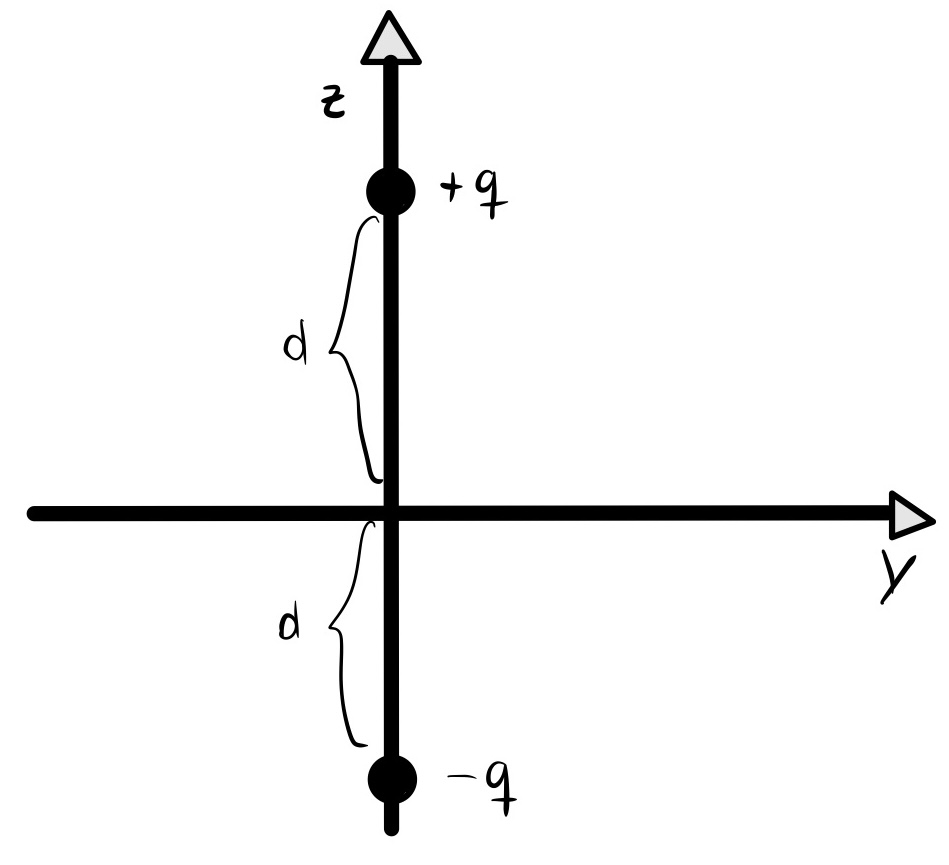
\includegraphics{IMG_3022.jpeg}
%\end{figure}

Imaginando uma carga puntiforme $q$ localizada próxima a um plano condutor infinito. A pergunta é: qual é o potencial elétrico em todos os pontos do espaço, levando em conta a presença do plano condutor? Para resolver esse problema com o Método das Imagens, criamos uma imagem fictícia da carga $q$ espelhada através do plano condutor. Suponha que a carga real q esteja a uma distância $d$ do plano condutor, em uma determinada direção. A imagem fictícia ($-q$) deve estar localizada simetricamente em relação ao plano, a uma distância $d$ do outro lado do plano.

Agora, temos duas cargas: a carga real $q$ e a imagem $-q$. A combinação dessas duas cargas e do plano condutor infinito satisfaz as condições de contorno. Isso ocorre porque o potencial gerado pela carga real e pelo potencial gerado pela carga fictícia (imagem) são cancelados exatamente na região do plano condutor, resultando em um potencial elétrico zero na superfície do condutor.

Sabendo o potencial poderíamos encontrar a densidade superficial de cargas $\sigma$ a partir da equação 

\begin{equation}
    \sigma = -\epsilon_{0} \frac{\partial V}{\partial n},
\end{equation}

consequentemente a carga total $Q$

\begin{equation}
    Q = \int \sigma da,
\end{equation}

e também poderíamos encontrar a força $F$ e a energia $W$, onde

\begin{equation}
    F = -\frac{1}{4\pi \epsilon_{0}} \frac{q^2}{(2d)^2}
\end{equation}

\begin{equation}
    W = -\frac{1}{4\pi \epsilon_{0}} \frac{q^2}{4d}. 
\end{equation}

E deve ser ressaltado que o método das imagens não serve somente para cargas pontuais, distribuição de cargas também podem ser espelhadas. 
